% !TEX root = slides.tex
%==============================================================================


%%%%%%%%%%%%%%%%%%%%%%%%%%%%%%%%%%%%%%%%%%%%%%%%%%%%%%%%%%
%%%%%%%%%%%%%%%%%%%%%%%%%%%%%%%%%%%%%%%%%%%%%%%%%%%%%%%%%%
%%%%%%%%%%%%%%%%%%%%%%%%%%%%%%%%%%%%%%%%%%%%%%%%%%%%%%%%%%


\begin{frame}[t]
\frametitle{Polynomial Chaos Representation of Augmented Input}


\centerline{
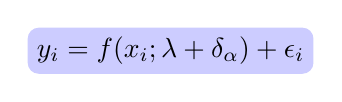
\begin{tikzpicture} \node [rounded corners,fill=blue!20] {
$y_i=f(x_i;\lambda+\delta_\alpha)+\epsilon_i$
};
\end{tikzpicture}
}

\bi
\item Zero-mean PC form $\delta_\alpha=\sum_{k=1}^{K} \alpha_k \Psi_k(\xi)$
\item Functional representation of a large class of random variables
\item The PC \emph{germ} $\xi$ is a standard random variable
\bi
\item e.g. Uniform$(-1,1)$ or Normal$(0,1)$
\ei
\item The PC bases (e.g. Legendre or Hermite polynomials) are orthogonal w.r.t. PDF of $\xi$
\[
\int \Psi_m(\xi)\Psi_k(\xi)\pi_\xi(\xi)d\xi=0 \quad\textrm{ for } m\neq k.
\]
\item PC representation allows efficient
\bi
\item Sampling
\item Moment estimation
\item Variance-based decomposition
\item Uncertainty propagation (via NISP)
\ei
\ei
\end{frame}

%%%%%%%%%%%%%%%%%%%%%%%%%%%%%%%%%%%%%%%%%%%%%%%%%%%%%%%%%%
% %%%%%%%%%%%%%%%%%%%%%%%%%%%%%%%%%%%%%%%%%%%%%%%%%%%%%%%%%%


% \begin{frame}[t]
% \frametitle{Non-intrusive Spectral Projection (NISP) for Uncertainty Propagation}

% \vspace*{-0.3cm}
% \bi
% \item Input random variable represented as PC
% \[
% \Lambda(\xi)=\sum_k \alpha_k \Psi_k(\xi)
% \]
% \item Black-box forward model $Z=f(\Lambda)$
% \item Seeking PC representation of output random variable
% \[
% Z(\xi)=\sum_k z_k \Psi_k(\xi)
% \]
% \item Use orthogonality property and quadrature integration to find PC coefficients
% \small
% \[
% z_k=\frac{1}{||\Psi_k||^2}\int f(\Lambda(\xi))\Psi_k(\xi)\pi_\xi(\xi) d\xi\approx \frac{1}{||\Psi_k||^2} \sum_q f(\Lambda(\xi^{(q)}))\Psi_k(\xi^{(q)}) w^{(q)}
% \]
% \ei

% \end{frame}